\documentclass[12pt, a4paper]{article}


% --- Pacotes Fundamentais ---
\usepackage[utf8]{inputenc}
\usepackage[T1]{fontenc}
\usepackage[brazil]{babel}
\usepackage{indentfirst} % Indenta o primeiro parágrafo de cada seção
\usepackage{graphicx}    % Inclusão de imagens
\usepackage{geometry}    % Configuração de margens
\usepackage{listings}    % Para incluir código fonte
\usepackage{xcolor}      % Cores para o código
\usepackage{url}         % Links e URLs
\usepackage{setspace}    % Para espaçamento entre linhas (1.5 é padrão ABNT)
\usepackage{float}       % Para posicionar figuras com [H]
\usepackage{pdfpages}    % Para incluir PDFs inteiros

% --- Configuração das Margens (Padrão ABNT) ---
\geometry{
    left=3cm,
    top=3cm,
    right=2cm,
    bottom=2cm
}

% --- Configuração de Cores para Código ---
\definecolor{codegreen}{rgb}{0,0.6,0}
\definecolor{codegray}{rgb}{0.5,0.5,0.5}
\definecolor{codepurple}{rgb}{0.58,0,0.82}
\definecolor{backcolour}{rgb}{0.95,0.95,0.92}

\lstset{
    backgroundcolor=\color{backcolour},   
    commentstyle=\color{codegreen},
    keywordstyle=\color{magenta},
    numberstyle=\tiny\color{codegray},
    stringstyle=\color{codepurple},
    basicstyle=\ttfamily\footnotesize,
    breakatwhitespace=false,         
    breaklines=true,                 
    captionpos=b,                    
    keepspaces=true,                 
    numbers=left,                    
    numbersep=5pt,                  
    showspaces=false,                
    showstringspaces=false,
    showtabs=false,                  
    tabsize=4,
    inputencoding=utf8,
    extendedchars=true,
    literate={á}{{\'a}}1 {à}{{\`a}}1 {ã}{{\~a}}1 {é}{{\'e}}1 {ê}{{\^e}}1 {í}{{\'i}}1 {ó}{{\'o}}1 {õ}{{\~o}}1 {ú}{{\'u}}1 {ç}{{\c{c}}}1 {Á}{{\'A}}1 {À}{{\`A}}1 {Ã}{{\~A}}1 {É}{{\'E}}1 {Ê}{{\^E}}1 {Í}{{\'I}}1 {Ó}{{\'O}}1 {Õ}{{\~O}}1 {Ú}{{\'U}}1 {Ç}{{\c{C}}}1
}

% --- Início do Documento ---
\begin{document}

% --- Capa Personalizada ---
\begin{titlepage}
    \begin{center}
        \textbf{\large UNIVERSIDADE DE SÃO PAULO - USP}\\
        \vspace{0.5cm}
        \textbf{\large INSTITUTO DE CIÊNCIAS MATEMÁTICAS E DE COMPUTAÇÃO - ICMC}\\
        \vspace{0.5cm}
        \textbf{\large SCC0540 – Base de Dados}\\
        \rule{\linewidth}{0.5mm}
        \vspace{3cm}
        
        \textbf{\Large Projeto - Cidades Inteligentes e Gestão de Dados Urbanos}\\
        \vspace{0.5cm}
        \textbf{\large Prontuário Eletrônico do Cidadão (PEC) no Contexto de Cidades Inteligentes}
        
        \vspace{3cm}
        
        \begin{flushright}
            \begin{minipage}{0.5\textwidth}
                \textbf{Integrantes:}\\
                Pedro Guilherme Tolvo - 10492012 \\
                Gabriel Henrique dos Santos - 13783972 \\
                Guilherme Ricardo Axhcar - 12563794 \\
                João Vitor Martins da Silva - 13696641 \\
                Luiz Henrique Benedito Belorio - 12563814 
                
                \vspace{1cm}
                \textbf{Docente:} Profª Drª Elaine Parros Machado de Sousa \\
                \textbf{Estagiário PAE:} Anderson Henrique Giacomini
            \end{minipage}
        \end{flushright}
        
        \vfill
        
        \textbf{São Carlos - SP}\\
        \textbf{Dezembro de 2025}
    \end{center}
\end{titlepage}

% --- Sumário ---
\tableofcontents
\newpage

% --- Conteúdo ---
\onehalfspacing 

% =========================================================================
% PARTE 1 e 2: DEFINIÇÃO E MODELAGEM
% =========================================================================

\section{Descrição do Problema e Requisitos de Dados}

A aplicação proposta se insere no contexto das cidades inteligentes, com foco na
área da saúde, auxiliando cidadãos e profissionais da saúde. Seu objetivo é centralizar,
organizar e disponibilizar informações clínicas de cidadãos em uma base de dados única
e segura, acessível por profissionais de saúde.
O sistema busca permitir que os profissionais de saúde tenham acesso rápido e
confiável ao histórico clínico dos pacientes, garantir a inclusão e a continuidade dos
tratamentos, otimizar a gestão de recursos em saúde, fornecer suporte à tomada de
decisão em políticas públicas. Entre as funcionalidades previstas destacam-se: cadastro
de cidadãos e profissionais da saúde. Sobre o paciente é possível a visualização de
consultas, exames, receitas, internações ou cirurgias. Os profissionais da saúde atuam
em uma ou mais unidades de saúde e acompanham pacientes em internação. A
internação é quando um cidadão permanece em uma ala hospitalar. Os médicos podem
realizar consultas e operar cirurgias. Os enfermeiros podem aplicar vacinas e auxiliar
cirurgias. As consultas cadastradas permitem saber o relatório médico, as receitas
indicadas e os exames que foram necessários. As unidades de saúde são onde os
cidadãos são consultados, elas são classificadas em unidades básicas de saúde e
hospitais. Nos hospitais ocorrem as cirurgias e as internações. Nas unidades básicas de
saúde são aplicadas as vacinas.

\section{Características, Atributos e Comportamento das Entidades}

\subsection*{Cidadão}
    O cidadão é um paciente que pode ser consultado diversas vezes 
    por qualquer médico em uma unidade de saúde, além disso, também 
    pode ser submetido a internações e cirurgias, tomar vacinas, 
    visualizar as receitas médicas e os exames realizados. 
    Ele é identificado por seu CPF e o sistema também mantém as 
    informações de nome, data de nascimento, sexo, endereço, contato, 
    tipo sanguíneo e alergias conhecidas.


\subsection*{Unidade de Saúde}
    É o local onde os cidadãos vão para se consultar e realizar outras ações, a
    depender do tipo da unidade, e onde os profissionais realizam essas operações. Cada
    unidade é identificada pelo CNES, e contém as demais informações: tipo, nome, endereço
    e horário de funcionamento. Ela se especializa nos dois tipos apresentados abaixo.

\paragraph{Unidade Básica de Saúde} 
    é a unidade para realização de atendimentos de
    atenção básica e integral, além da aplicação de vacinas.

\paragraph{Hospital} 
    é uma unidade destinada à realização de cirurgias e internações. Serão
    armazenadas informações de capacidade de pacientes e situação de
    lotação.

\subsection*{Profissional de Saúde}
    Cada profissional atua em uma ou mais unidades de saúde obedecendo seu nível
    de especialização. Cada um é identificado por um CPF e possui nome, tipo e número de
    registro em seu respectivo órgão de classe - CRM ou COREN, a depender de sua
    formação. Podendo se ramificar em dois tipos dentro do escopo do projeto:

\paragraph{Médico}
    É o profissional responsável pela realização de consultas, pela
    solicitação, execução de exames e condução de cirurgias, o responsável
    pela consulta, não necessariamente, realiza o exame ou a cirurgia. Esse
    profissional pode possuir uma especialidade médica vinculada ao seu
    cadastro. Todo médico possui um registro ativo junto ao CRM.

\paragraph{Enfermeiros} 
    É o profissional responsável por auxiliar em cirurgias e aplicar
    vacinas. Todo enfermeiro deve possuir um registro ativo junto ao COREN.

\subsection*{Consulta}
    A consulta se dá entre um paciente e um médico em uma determinada data, a
    consulta também ocorre em uma unidade de saúde. Cada consulta deve ser registrada
    com a data do atendimento e relatório médico. Cada consulta pode gerar uma ou mais
    receitas e também é possível a emissão de pedidos de exames, quando necessário.

\subsection*{Receita}
    A partir de uma consulta, poderá ser indicado uma receita que é identificada pelo
    medicamento indicado com suas respectivas dosagens e a duração do tratamento.

\subsection*{Exame}
    O exame é solicitado durante uma consulta. Ele possui informações sobre o tipo
    do exame (laboratorial, imagem, etc.), a data de realização, local onde será/foi realizado,
    o resultado obtido através de um link.

\subsection*{Vacinação e Vacinas}
    A vacinação faz parte do histórico de imunização do cidadão e inclui informações
    sobre a vacina e dose aplicadas, data de aplicação, unidade básica de saúde
    responsável pelo armazenamento do imunizante, o enfermeiro responsável pela aplicação
    e o cidadão que tomou a vacina. As vacinas são identificadas por um lote e código de
    vacina e tem as informações de nome popular, fabricante e validade.

    O cidadão toma uma dose de qualquer vacina em uma unidade de saúde. Além
    disso, a unidade de saúde e uma dose para vacina pode ser aplicada em diversos
    cidadãos e em uma unidade de saúde, o cidadão consegue tomar vários tipos de vacinas.

\subsection*{Cirurgia}
    A cirurgia é um procedimento especial realizado em hospital, envolvendo um ou
    mais médicos na operação, enfermeiro(s) em seu auxílio e ao qual o cidadão será
    submetido. São registrados o nome do procedimento, a duração e data de realização do
    procedimento, observações médicas e cuidados posteriores necessários.

\subsection*{Internação}
    A internação representa a permanência do paciente em uma ala hospitalar e é
    realizado durante esse tempo o acompanhamento de profissionais da saúde e contém
    informações sobre a data de entrada, a data de alta, motivo da internação e em qual ala
    hospitalar está residindo o enfermo.

\subsection*{Acompanhamento}
    Durante a internação, o cidadão vai ser submetido ao período de acompanhamento
    por um ou mais profissionais da saúde, onde durante esse período ele pode ser sujeito a
    procedimentos e a averiguação da condição no mesmo, armazenando informações de
    hora e data do acompanhamento.

\section{Relacionamentos entre as Entidades}
\begin{enumerate}
    \item \textbf{Aplica:} Um enfermeiro pode aplicar N vacinações, a vacinação é aplicada por 1 enfermeiro. (Enfermeiro 1:N Vacinação).
    
    \item \textbf{Atua:} Um profissional de saúde atua em N unidades de saúde e uma unidade de saúde pode ter N profissionais de saúde atuando nela. (Profissional N:N Unidade de Saúde).
    
    \item \textbf{Consulta:} Um cidadão pode se consultar com N médicos, um médico pode consultar N cidadãos. (Cidadão N:N Médicos).
    
    \item \textbf{Atende:} Um profissional da saúde atende N internações, uma internação é atendida por N profissionais da saúde. (Profissional N:N Internação).
    
    \item \textbf{Auxilia:} Um enfermeiro auxilia N cirurgias, uma cirurgia pode ser auxiliada por N enfermeiros. (Enfermeiro N:N Cirurgia).
    
    \item \textbf{Opera:} Um ou mais médicos podem operar em N cirurgias e uma cirurgia é operada por N médicos. (Médico N:N Cirurgia).
    
    \item \textbf{Ocorre:} Uma consulta pode ocorrer em uma unidade de saúde e em uma unidade de saúde ocorrem N Consultas. (Consulta N:1 Unidade de saúde).
    
    \item \textbf{Abriga (2 relações diferentes):}
    \begin{enumerate}
        \item Uma internação pode ser abrigada somente em um hospital, um hospital pode abrigar N internações. (Hospital 1:N Internações).
        \item Uma cirurgia pode ser abrigada em somente um hospital, um hospital pode abrigar N cirurgias. (Hospital 1:N Cirurgias).
    \end{enumerate}
    
    \item \textbf{Gera (2 relações diferentes):}
    \begin{enumerate}
        \item Uma consulta pode gerar vários exames, um exame é gerado por somente uma consulta. (Consulta 1:N Exames).
        \item Uma consulta pode gerar várias receitas, uma receita é gerada por somente uma consulta. (Consulta 1:N Receita).
    \end{enumerate}
\end{enumerate}

\section{Restrições de Integridade}
\begin{itemize}
    \item \textbf{Cidadão}
    \begin{itemize}
        \item \textbf{Integridade de Entidade (Chave Primária):}
        \begin{itemize}
            \item Deve ser identificado unicamente pelo CPF. Não podem existir dois cidadãos com o mesmo CPF.
        \end{itemize}
        \item \textbf{Integridade de Domínio (Valores Válidos):}
        \begin{itemize}
            \item Data de Nascimento: Deve ser uma data válida e no passado.
            \item Sexo, Tipo Sanguíneo: Devem pertencer a uma lista de valores predefinidos (ex: 'Masculino'/'Feminino'/'Outro'; 'A+'/'A-'/'B+' etc.).
            \item CPF: Deve seguir o formato e algoritmo de validação padrão.
        \end{itemize}
        \item \textbf{Regras de Negócio (Integridade Semântica):}
        \begin{itemize}
            \item A exclusão de um cidadão não deve apagar o registro do banco de dados, mas sim desativar, para preservar todo o histórico clínico associado.
        \end{itemize}
    \end{itemize}

    \item \textbf{Profissional de Saúde (e especializações Médico/Enfermeiro)}
    \begin{itemize}
        \item \textbf{Integridade de Entidade (Chave Primária):}
        \begin{itemize}
            \item Deve ser identificado unicamente pelo CPF.
        \end{itemize}
        \item \textbf{Integridade de Domínio (Valores Válidos):}
        \begin{itemize}
            \item Tipo: O valor deve ser restrito a 'Médico' ou 'Enfermeiro', conforme o escopo do projeto.
            \item CRM: Obrigatório e em formato válido se o Tipo for 'Médico'.
            \item COREN: Obrigatório e em formato válido se o Tipo for 'Enfermeiro'.
        \end{itemize}
    \end{itemize}

    \item \textbf{Unidade de Saúde (e especializações Hospital/Unidade Básica)}
    \begin{itemize}
        \item \textbf{Integridade de Entidade (Chave Primária):}
        \begin{itemize}
            \item Deve ser identificada unicamente pelo CNES (Cadastro Nacional de Estabelecimentos de Saúde).
        \end{itemize}
        \item \textbf{Integridade de Domínio (Valores Válidos):}
        \begin{itemize}
            \item Tipo: O valor deve ser restrito a 'Unidade Básica de Saúde' ou 'Hospital'.
            \item Horário de Funcionamento: Deve seguir um formato de texto ou de tempo válido.
        \end{itemize}
    \end{itemize}

    \item \textbf{Consulta}
    \begin{itemize}
        \item \textbf{Integridade de Entidade (Chave Primária):}
        \begin{itemize}
            \item A chave primária deve ser composta, formada pelas chaves estrangeiras de Cidadão, Médico e pela Data da consulta para garantir sua unicidade.
        \end{itemize}
        \item \textbf{Integridade Referencial (Chaves Estrangeiras):}
        \begin{itemize}
            \item Deve estar obrigatoriamente ligada a um Cidadão e um Médico válidos e existentes.
        \end{itemize}
        \item \textbf{Integridade de Domínio (Valores Válidos):}
        \begin{itemize}
            \item Data da Consulta: Não pode ser uma data inválida ou inconsistente.
        \end{itemize}
        \item \textbf{Regras de Negócio (Integridade Semântica):}
        \begin{itemize}
            \item Para que o cidadão faça a consulta é necessário que a consulta esteja vinculada a uma unidade de saúde e atendida por um médico que trabalhe nesse mesmo local.
        \end{itemize}
    \end{itemize}

    \item \textbf{Receita}
    \begin{itemize}
        \item \textbf{Integridade de Entidade (Chave Primária):}
        \begin{itemize}
            \item É uma entidade fraca. Sua chave primária é composta pela chave primária da Consulta (que a gerou) e pelo atributo Medicamento.
        \end{itemize}
        \item \textbf{Integridade Referencial (Chaves Estrangeiras):}
        \begin{itemize}
            \item Deve obrigatoriamente estar ligada a uma Consulta existente.
        \end{itemize}
        \item \textbf{Integridade de Domínio (Valores Válidos):}
        \begin{itemize}
            \item Dosagem e Duração do Tratamento: Devem seguir formatos predefinidos.
        \end{itemize}
        \item \textbf{Regras de Negócio (Integridade Semântica):}
        \begin{itemize}
            \item Só pode ser gerada a partir de uma Consulta.
        \end{itemize}
    \end{itemize}

\item \textbf{Exame}
    \begin{itemize}
        \item \textbf{Integridade de Entidade (Chave Primária):}
        \begin{itemize}
            \item É uma entidade fraca. Sua chave primária é composta pela chave primária da Consulta (que o solicitou) e pelo atributo Tipo do Exame.
        \end{itemize}
        \item \textbf{Integridade Referencial (Chaves Estrangeiras):}
        \begin{itemize}
            \item Deve obrigatoriamente estar ligado a uma Consulta existente.
        \end{itemize}
        \item \textbf{Integridade de Domínio (Valores Válidos):}
        \begin{itemize}
            \item Tipo do Exame: Pode ser uma lista de valores (ex: 'laboratorial', 'imagem').
            \item Link do Resultado: Deve ser um formato de URL válido.
            \item Data de Realização: Deve ser uma data válida.
        \end{itemize}
        \item \textbf{Regras de Negócio (Integridade Semântica):}
        \begin{itemize}
            \item Só pode ser gerada a partir de uma Consulta.
        \end{itemize}
    \end{itemize}

    \item \textbf{Vacina}
    \begin{itemize}
        \item \textbf{Integridade de Entidade (Chave Primária):}
        \begin{itemize}
            \item Sua chave primária é composta pela combinação de lote e código de vacina.
        \end{itemize}
        \item \textbf{Integridade de Domínio (Valores Válidos):}
        \begin{itemize}
            \item Validade: Deve ser uma data válida.
        \end{itemize}
    \end{itemize}

    \item \textbf{Vacinação (Evento)}
    \begin{itemize}
        \item \textbf{Integridade de Entidade (Chave Primária):}
        \begin{itemize}
            \item É uma entidade associativa. Sua chave primária é composta pela chave do Cidadão e chave da Vacina.
        \end{itemize}
        \item \textbf{Integridade Referencial (Chaves Estrangeiras):}
        \begin{itemize}
            \item Deve estar ligada a um Cidadão, uma Vacina, um Enfermeiro e uma Unidade Básica de Saúde existentes.
        \end{itemize}
        \item \textbf{Integridade de Domínio (Valores Válidos):}
        \begin{itemize}
            \item Dose, Lote e Data de Aplicação devem ser registrados.
        \end{itemize}
        \item \textbf{Regras de Negócio (Integridade Semântica):}
        \begin{itemize}
            \item Para que exista uma vacinação é necessário que a Unidade Básica de Saúde seja a mesma que o Enfermeiro está vinculado.
        \end{itemize}
    \end{itemize}

    \item \textbf{Cirurgia}
    \begin{itemize}
        \item \textbf{Integridade de Entidade (Chave Primária):}
        \begin{itemize}
            \item É uma entidade fraca. Sua chave primária pode ser composta pela chave do Cidadão, do Hospital e a Data de Realização.
        \end{itemize}
        \item \textbf{Integridade Referencial (Chaves Estrangeiras):}
        \begin{itemize}
            \item Deve ocorrer em um Hospital e estar ligada a um Cidadão.
        \end{itemize}
        \item \textbf{Integridade de Domínio (Valores Válidos):}
        \begin{itemize}
            \item Duração: Deve ser um formato de tempo/intervalo.
            \item Data de Realização: Deve ser uma data e hora válidas.
        \end{itemize}
        \item \textbf{Regras de Negócio (Integridade Semântica):}
        \begin{itemize}
            \item Para garantir a consistência é necessário que o(s) médico(s) e o(s) enfermeiro(s) estejam ligados ao mesmo Hospital que a cirurgia está sendo realizada.
        \end{itemize}
    \end{itemize}

    \item \textbf{Internação}
    \begin{itemize}
        \item \textbf{Integridade de Entidade (Chave Primária):}
        \begin{itemize}
            \item É uma entidade fraca. Sua chave primária é composta pela chave do Cidadão, do Hospital e da Data de Entrada.
        \end{itemize}
        \item \textbf{Integridade Referencial (Chaves Estrangeiras):}
        \begin{itemize}
            \item Deve estar ligada a um Cidadão e a um Hospital.
        \end{itemize}
        \item \textbf{Integridade de Domínio (Valores Válidos):}
        \begin{itemize}
            \item Data de Entrada e Data de Alta: Devem ser datas válidas.
        \end{itemize}
        \item \textbf{Regras de Negócio (Integridade Semântica):}
        \begin{itemize}
            \item A Data de Alta não pode ser anterior à Data de Entrada.
        \end{itemize}
    \end{itemize}

    \item \textbf{Acompanhamento}
    \begin{itemize}
        \item \textbf{Integridade de Entidade (Chave Primária):}
        \begin{itemize}
            \item É uma entidade gerada a partir de uma agregação, dependente de Internação e Profissional. Sua chave é composta pela chave da Internação, a chave do Profissional e a Data/Hora do Acompanhamento.
        \end{itemize}
        \item \textbf{Integridade Referencial (Chaves Estrangeiras):}
        \begin{itemize}
            \item Deve estar ligado a uma Internação e a Profissionais de Saúde válidos.
        \end{itemize}
        \item \textbf{Integridade de Domínio (Valores Válidos):}
        \begin{itemize}
            \item Hora e Data do Acompanhamento: Devem ter formatos válidos.
        \end{itemize}
        \item \textbf{Regras de Negócio (Integridade Semântica):}
        \begin{itemize}
            \item Para que exista o acompanhamento é necessário que o cidadão e o profissional de saúde estejam vinculados (internado e atua respectivamente) a uma mesma unidade de saúde.
            \item A data/hora do acompanhamento deve estar entre a data de entrada e a data de alta da internação.
        \end{itemize}
    \end{itemize}
\end{itemize}

\section{Principais Operações (Funcionalidades)}
\begin{description}
    \item[A. Cadastro:] Cidadãos, profissionais de saúde, unidades de saúde, consultas, receitas, exames, vacinas, internações, vacinações, acompanhamentos e cirurgias.
    
    \item[B. Atualização:] Dados cadastrais de cidadãos, profissionais, unidades e resultados de exames.
    
    \item[C. Consulta:] Histórico clínico completo do paciente; vacinas em atraso por faixa etária; consultas por unidade de saúde em determinado período; profissionais por especialidade; histórico de procedimentos realizados por profissional ou unidade de atendimento; pacientes com prescrição de determinados medicamentos; exames solicitados, realizados e pendentes; taxas de internação por bairro ou faixa etária; doenças mais registradas por região; relatórios de consumo de medicamentos; tempo médio entre solicitação e entrega de exames.
    
    \item[D. Remoção lógica:] Inativação de registros antigos sem perda do histórico.
\end{description}

\section{Modelo Entidade-Relacionamento (MER)}
Abaixo apresentamos o diagrama conceitual do banco de dados:

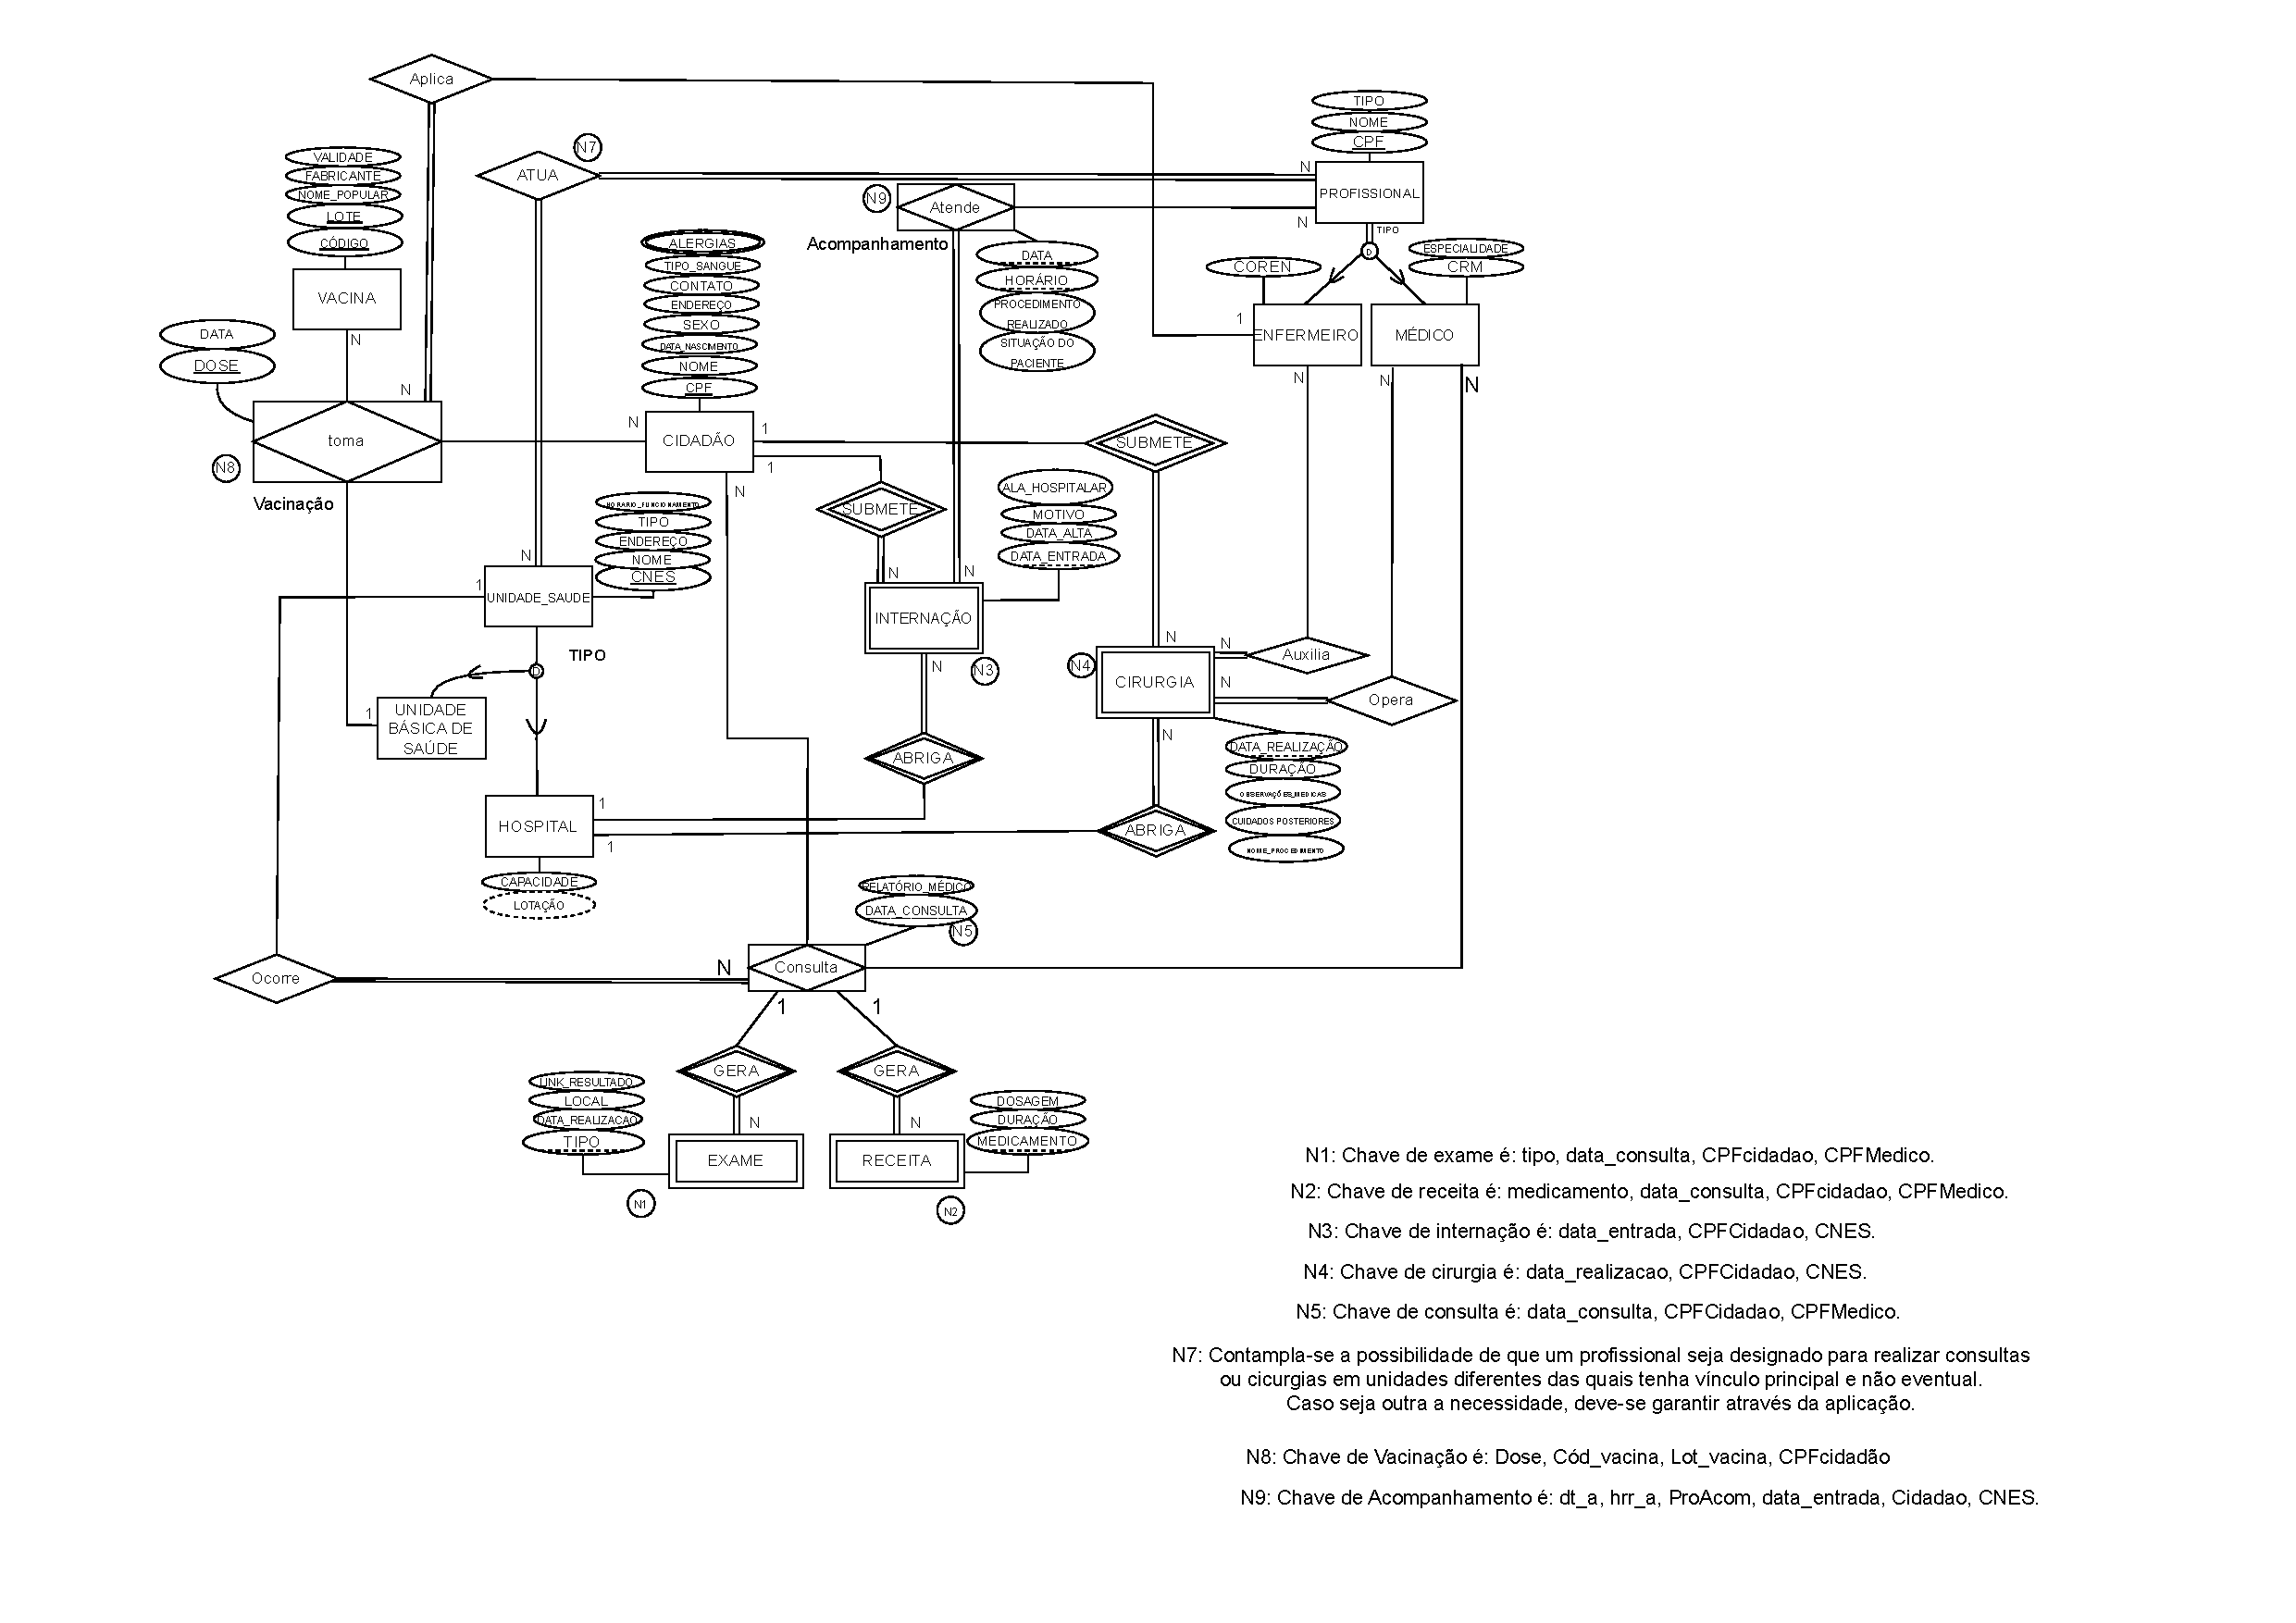
\includepdf[pages={1}, width=\paperwidth, pagecommand={}]{MER.pdf}

\section{Alterações realizadas na segunda parte do projeto}
Para a segunda parte do projeto, por recomendação do monitor e visando a normalização adequada, foram realizados ajustes nas entidades fracas e na tabela de relacionamento de médicos e unidades.

\section{Modelo Relacional}
Abaixo apresentamos o diagrama relacional do banco de dados:

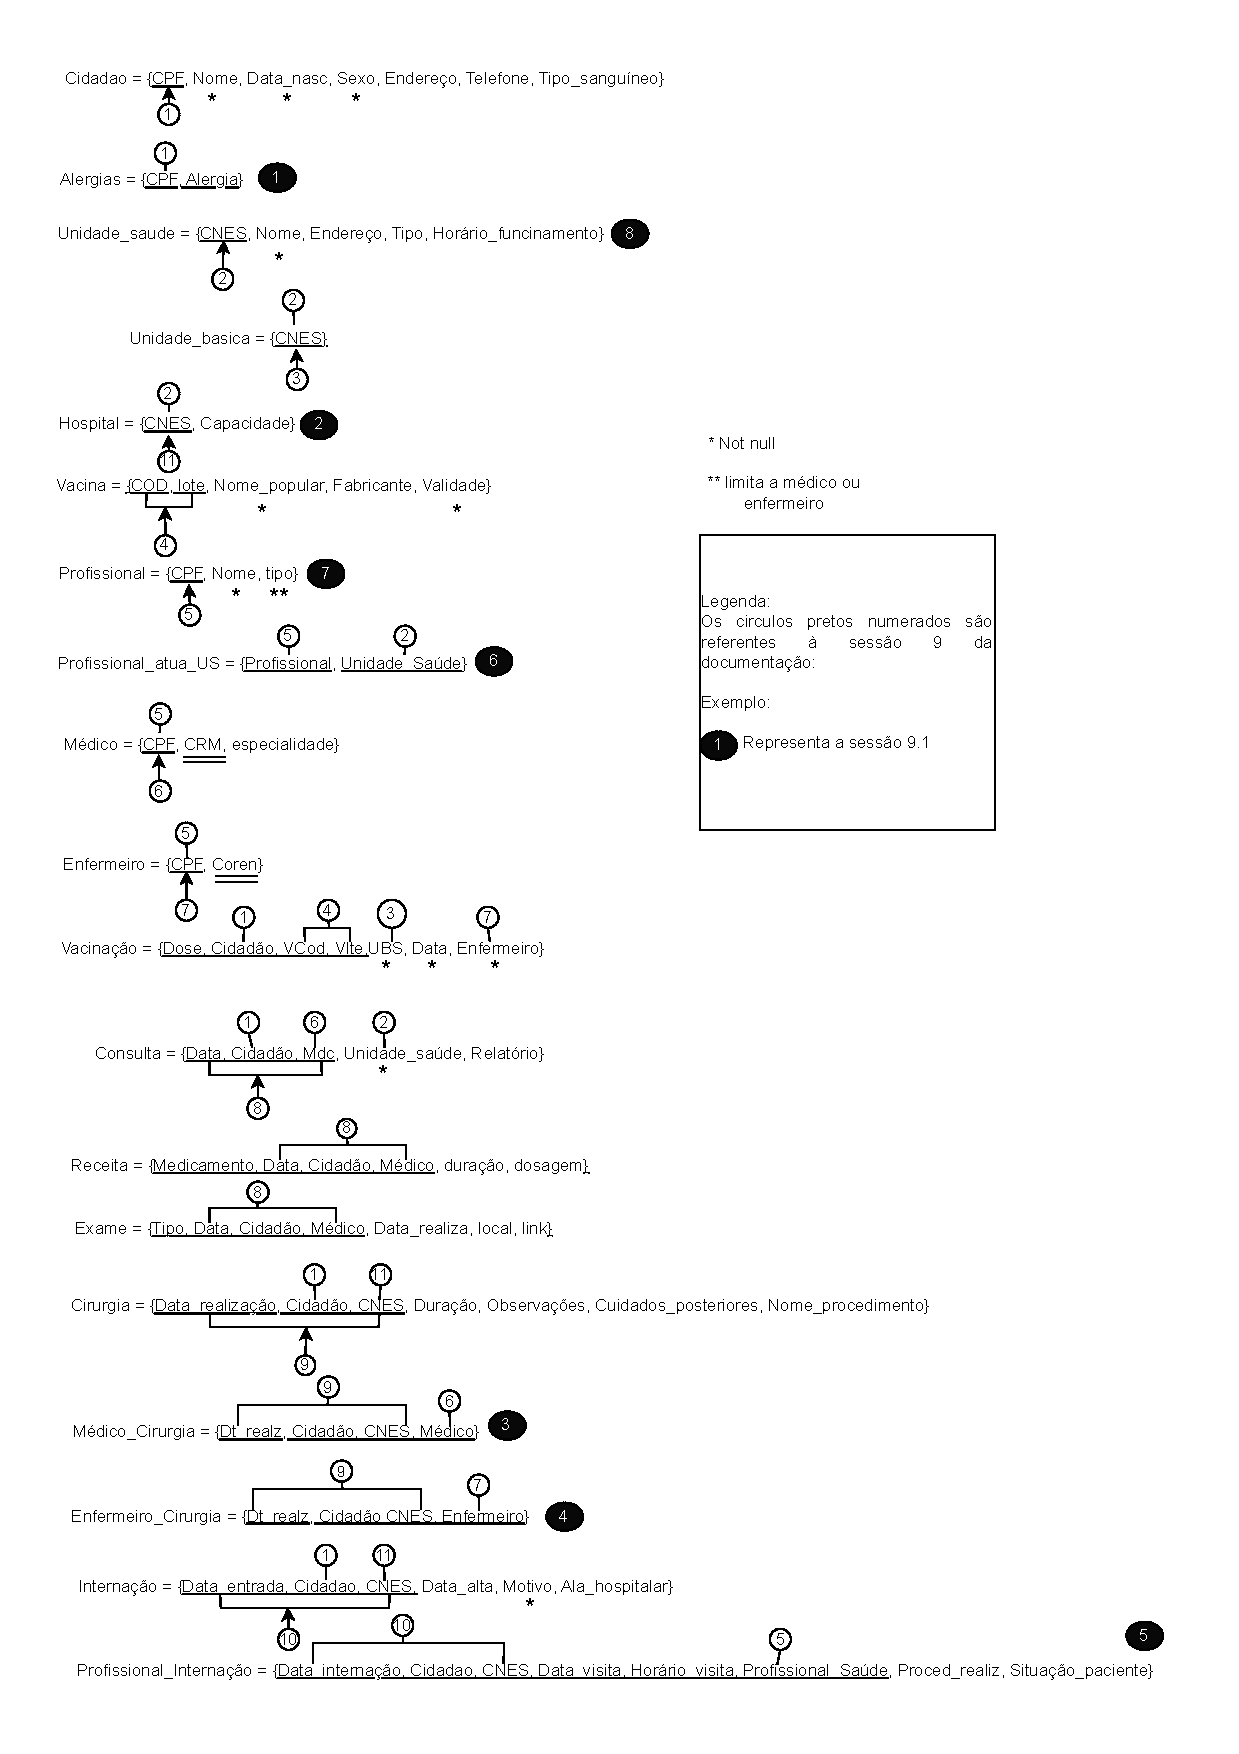
\includepdf[pages={1}, width=\paperwidth, pagecommand={}]{relacional.pdf}

\subsection{Notes}
\begin{description}
    \item[Consulta:] Deve estar obrigatoriamente ligada a um Cidadão e um Médico válidos e existentes.
    
    \item[Receita:] Deve obrigatoriamente estar ligada a uma Consulta existente.
    
    \item[Exame:] Deve obrigatoriamente estar ligado a uma Consulta existente.
    
    \item[Vacinação:] Deve estar ligada a um Cidadão, uma Vacina, um Enfermeiro e uma Unidade Básica de Saúde existentes.
    
    \item[Cirurgia:] Deve ocorrer em um Hospital e estar ligada a um Cidadão.
    
    \item[Internação:] Deve estar ligada a um Cidadão e a um Hospital.
    
    \item[Acompanhamento:] Deve estar ligado a uma Internação e a Profissionais de Saúde válidos.
\end{description}

\section{Justificativas para o Modelo Relacional}
A seguir estão listadas as justificativas tomadas para a criação do modelo
relacional utilizando o modelo entidade relacionamento desenvolvido no tópico anterior.

\subsection{Atributo Multivalorado da entidade Cidadão}
\begin{itemize}
    \item \textbf{Solução adotada:} Mapeou-se o atributo multivalorado Alergias como uma tabela nova,
        tendo como conteúdo o CPF do cidadão como chave estrangeira e a alergia em questão.

    \item \textbf{Vantagem:} Esse mapeamento garante que não exista incoerências com o
        armazenamento do atributo Alergias e com uma consulta temos o retorno de todas as
        alergias que um cidadão possui.

    \item \textbf{Desvantagem:} Aumenta o custo computacional, ao gerar mais uma junção 
    nas consultas e mais uma tabela para ser feito dentro do sistema

    \item \textbf{Solução alternativa:} O mapeamento de atributos multivalorados também torna possível 
    mapeá-lo na tabela da entidade a qual ele pertence, porém é possível que um cidadão tenha diversas alergias, 
    gerando assim, uma necessidade de estipular um tamanho máximo para este atributo que em suma maioria seria 
    muito pouco utilizado, além da possibilidade de permitir incoerências.
\end{itemize}

\subsection{Atributo Derivado da entidade Hospital}
\begin{itemize}
    \item \textbf{Solução adotada:} A solução adotada foi que será calculado sob demanda, considerou-se
que não é uma informação de alta demanda (várias vezes ao dia) mas sim uma
informação que será consultada no máximo uma vez por dia (logo pela manhã) e assim
com essa informação já em mãos, o usuário conseguirá manejar as internações para que
não falte espaço no hospital.

    \item \textbf{Vantagem:} O custo de armazenamento é menor, já que essa informação não ficará
armazenada no banco de dados e não precisará de atualizações para cada internação
inserida/removida.

    \item \textbf{Desvantagem:} Na hora de fazer a consulta, será necessário varrer tanto a tabela de
lotação e de internação toda vez.

    \item \textbf{Solução alternativa:} Criar um atributo para lotação dentro da entidade Hospital, onde a
cada registro e remoção de internação resultaria em incrementar ou decrementar o
atributo lotação.

\end{itemize}

\subsection{Relacionamento “Auxilia”, Cirurgia - Enfermeiro (N:N)}
\begin{itemize}
    \item \textbf{Situação:} A entidade Cirurgia possui participação total no relacionamento Auxilia com a
entidade Enfermeiro, porém não é possível garantir a participação total no modelo
relacional.

    \item \textbf{Solução:} A participação total será tratada na aplicação.

\end{itemize}

\subsection{Relacionamento “Opera”, Cirurgia - Médico (N:N)}
\begin{itemize}
    \item \textbf{Situação:} A entidade Cirurgia possui participação total no relacionamento Opera com a
entidade Médico, porém não é possível garantir a participação total no modelo relacional.

    \item \textbf{Solução:} A participação total será tratada na aplicação.

\end{itemize}

\subsection{Relacionamento “Atende”, Internação - Profissional (N:N)}
\begin{itemize}
    \item \textbf{Situação:} A entidade Internação possui participação total no relacionamento Atende com
a entidade Profissional, porém o próprio relacionamento não foi mapeado mas sim a
agregação “Acompanhamento”, contendo as chaves estrangeiras das tabelas geradoras.
Mas, por ser originalmente um relacionamento N:N não é possível garantir a participação
total de internação no modelo relacional.

    \item \textbf{Solução:} A participação total será tratada na aplicação.

\end{itemize}

\subsection{Relacionamento “atua”, Unidade de saúde - Profissional (N : N)}
\begin{itemize}
    \item \textbf{Situação:} Por se tratar de um relacionamento N:N, foi feito o mapeamento entre as duas
entidades, criando uma terceira tabela “atua” para representar quais unidades de saúde
um profissional atua. Tanto a entidade unidade de saúde quanto o profissional fazem
participação total.

    \item \textbf{Solução:} A participação total será tratada na aplicação.

\end{itemize}

\subsection{Generalização/Especialização Profissional}
\begin{itemize}
    \item \textbf{Solução adotada:} Mapeou-se a tabela Profissional e as suas respectivas
especializações, uma vez que a entidade generalista possuí relacionamentos com outras
entidades e possui poucas entidades específicas.

    \item \textbf{Vantagem:} As consultas se concentram mais nas entidades específicas, maior
consistência de dados, uma vez que na tabela generalista não terá dados de tipos
diferentes.

    \item \textbf{Desvantagem:} Não garante a especialização total de profissional em enfermeiro ou
médico. Necessidade de uma junção a mais para buscar informações básicas de
enfermeiro/médico.

    \item \textbf{Solução alternativa:} Mapear tudo em uma só tabela “Profissional” e fazer as relações a
partir dela. Porém, o número de nulos aumentaria por conter tanto informações de
enfermeiro quanto de médicos. E cada relacionamento da entidade generalista teria que
ser aplicado para cada uma das entidades especializadas.

\end{itemize}

\subsection{Generalização/Especialização Unidade Saúde}
\begin{itemize}
    \item \textbf{Solução adotada:} A entidade unidade saúde possui um relacionamento de
especialização disjunta para evitar que uma unidade seja ao mesmo tempo básica e
hospital.

    \item \textbf{Vantagem:} Garante a especialização parcial de unidade saúde, maior consistência de
dados já que os atributos das específicas não estão na tabela generalista.

    \item \textbf{Desvantagem:} O mapeamento da generalização implica na complicação das consultas e
junções, onde buscar dados de unidade de saúde ou hospital com informações básicas
seria necessário fazer JOINS.

    \item \textbf{Solução alternativa:} Uma opção seria tratar os atributos de unidade básica de saúde e
hospital como valores de atributo dentro da entidade unidade saúde, sem a necessidade de trabalhar com mais duas tabelas para isso.

\end{itemize}

\newpage

% =========================================================================
% PARTE 3: IMPLEMENTAÇÃO E CONSULTAS 
% =========================================================================
\section{Implementação e Implantação}

Esta seção descreve os detalhes técnicos do desenvolvimento do sistema Prontuário Eletrônico do Cidadão (PEC), incluindo as ferramentas utilizadas, a arquitetura da solução e os principais trechos de código SQL desenvolvidos, conforme solicitado nos requisitos do projeto.

\subsection{Tecnologias e Ferramentas}
Para atender aos requisitos de portabilidade e robustez, o sistema foi desenvolvido utilizando as seguintes tecnologias:

\begin{itemize}
    \item \textbf{SGBD:} PostgreSQL (Versão 13).
    \item \textbf{Linguagem Backend:} Python 3.9 com framework Flask.
    \item \textbf{Driver de Banco de Dados:} Biblioteca \texttt{psycopg2} para conexão e prevenção de injeção de SQL.
    \item \textbf{Ambiente:} Docker e Docker Compose para orquestração dos containers de banco, backend e frontend.
\end{itemize}

\subsection{Requisitos de Sistema}
O sistema foi projetado para rodar sobre a plataforma \textbf{Docker}. Portanto, o único requisito de sistema é um ambiente (Windows, Linux ou macOS) com o \textit{Docker Engine} e \textit{Docker Compose} instalados e configurados.

\subsection{Trechos de Código e Consultas SQL}
Abaixo são apresentadas as implementações SQL das funcionalidades mais críticas do sistema.

% 1. Divisão Relacional
\subsubsection{Relatório de Vacinação Completa (Divisão Relacional)}
\textbf{Descrição:} Identifica cidadãos que receberam \textbf{todos} os tipos de vacinas cadastradas. A lógica utiliza \texttt{NOT EXISTS} com \texttt{EXCEPT} para encontrar cidadãos para os quais não existe nenhuma vacina pendente.

\noindent\textbf{Localização:}
\begin{itemize}
    \item \textbf{Arquivo:} \texttt{src/back/queries/consultas\_queries.py}
    \item \textbf{Função:} \texttt{get\_cidadaos\_todas\_vacinas\_query()}
\end{itemize}

\begin{lstlisting}[language=SQL, caption=Divisão Relacional: Cidadãos com todas as vacinas]
SELECT c.cpf, c.nome
FROM cidadao c
WHERE NOT EXISTS (
    -- Seleciona todas as vacinas disponiveis
    SELECT v.lote, v.cod FROM vacina v
    EXCEPT
    -- Remove as vacinas que o cidadao ja tomou
    SELECT vac.vacina_lote, vac.vacina_cod
    FROM vacinacao vac
    WHERE vac.cidadao = c.cpf
)
ORDER BY c.nome
\end{lstlisting}

% 2. Histórico Unificado
\subsubsection{Prontuário Unificado do Paciente}
\textbf{Descrição:} Constrói o histórico cronológico de um paciente agregando consultas, exames e receitas. Utiliza múltiplos \texttt{LEFT JOIN} para garantir o retorno de dados parciais (ex: consulta sem receita).

\noindent\textbf{Localização:}
\begin{itemize}
    \item \textbf{Arquivo:} \texttt{src/back/queries/consultas\_queries.py}
    \item \textbf{Função:} \texttt{get\_historico\_cidadao\_query()}
\end{itemize}

\begin{lstlisting}[language=SQL, caption=Histórico Médico com Múltiplas Junções]
SELECT
    c.nome as cidadao,
    cons.data as data_consulta,
    cons.relatorio as relatorio_medico,
    e.tipo as tipo_exame,
    r.medicamento
FROM cidadao c
LEFT JOIN consulta cons ON c.cpf = cons.cidadao
LEFT JOIN exame e ON cons.cidadao = e.cidadao 
    AND cons.medico = e.medico AND cons.data = e.data
LEFT JOIN receita r ON cons.cidadao = r.cidadao 
    AND cons.medico = r.medico AND cons.data = r.data
WHERE c.cpf = %s 
ORDER BY cons.data DESC NULLS LAST
\end{lstlisting}

% 3. Agregação
\subsubsection{Relatório de Consultas por Unidade}
\textbf{Descrição:} Consulta analítica que contabiliza o total de atendimentos realizados por cada unidade de saúde em um determinado período.

\noindent\textbf{Localização:}
\begin{itemize}
    \item \textbf{Arquivo:} \texttt{src/back/queries/consultas\_queries.py}
    \item \textbf{Função:} \texttt{get\_consultas\_unidade\_query()}
\end{itemize}

\begin{lstlisting}[language=SQL, caption=Agregação: Total de consultas por Unidade]
SELECT 
    u.nome as unidade, 
    COUNT(*) as numero_consultas
FROM unidade_saude u
JOIN consulta cons ON u.cnes = cons.unidade_saude
WHERE cons.data BETWEEN %s AND %s
GROUP BY u.cnes, u.nome
ORDER BY numero_consultas DESC
\end{lstlisting}

% 4. Subconsulta Correlacionada (Vacinas em Atraso)
\subsubsection{Relatório de Vacinas em Atraso}
\textbf{Descrição:} Identifica cidadãos que deveriam ter tomado uma vacina específica (baseado na idade/data de nascimento), mas ainda não possuem o registro de vacinação correspondente. Utiliza uma subconsulta correlacionada com \texttt{NOT EXISTS}.

\noindent\textbf{Localização:}
\begin{itemize}
    \item \textbf{Arquivo:} \texttt{src/back/queries/consultas\_queries.py}
    \item \textbf{Função:} \texttt{get\_vacinas\_atraso\_query()}
\end{itemize}

\begin{lstlisting}[language=SQL, caption=Subconsulta: Vacinas Pendentes por Idade]
SELECT c.cpf, c.nome, c.data_nasc
FROM cidadao c
WHERE c.data_nasc > %s -- Data corte para a vacina
AND NOT EXISTS (
    SELECT 1 FROM vacinacao v
    WHERE v.cidadao = c.cpf AND v.vacina_cod = %s
)
ORDER BY c.data_nasc DESC
\end{lstlisting}

% 5. Filtro de Texto (ILIKE) e Distinct
\subsubsection{Pacientes por Medicamento Prescrito}
\textbf{Descrição:} Lista pacientes que receberam prescrição de um determinado medicamento. Utiliza \texttt{DISTINCT} para evitar duplicatas (caso o paciente tome o remédio recorrentemente) e \texttt{ILIKE} para busca textual flexível (case-insensitive).

\noindent\textbf{Localização:}
\begin{itemize}
    \item \textbf{Arquivo:} \texttt{src/back/queries/consultas\_queries.py}
    \item \textbf{Função:} \texttt{get\_pacientes\_medicamento\_query()}
\end{itemize}

\begin{lstlisting}[language=SQL, caption=Filtro Textual: Busca de Pacientes por Remédio]
SELECT DISTINCT c.cpf, c.nome, r.medicamento, r.dosagem, r.duracao
FROM cidadao c
JOIN receita r ON c.cpf = r.cidadao
WHERE r.medicamento ILIKE %s
ORDER BY c.nome
\end{lstlisting}

\subsection{Segurança (SQL Injection)}
Para cumprir o requisito de segurança, todas as rotas utilizam consultas parametrizadas.

\noindent\textbf{Localização:}
\begin{itemize}
    \item \textbf{Arquivo:} \texttt{src/back/routes/cidadao.py}
    \item \textbf{Rotina:} \texttt{buscar\_cidadao\_completo(cpf)}
\end{itemize}

\begin{lstlisting}[language=Python, caption=Exemplo de Chamada Segura com Psycopg2]
# O uso da tupla (cpf,) garante que o driver trate o dado
cur.execute(get_cidadao_basic_query(), (cpf,))
\end{lstlisting}

\section{Conclusão}

O desenvolvimento do projeto Prontuário Eletrônico do Cidadão (PEC) permitiu consolidar, de forma prática, os conceitos teóricos de banco de dados abordados na disciplina. A transição da modelagem conceitual para a implementação física exigiu não apenas o domínio da linguagem SQL, mas também uma compreensão sistêmica de como garantir a integridade e a consistência dos dados em uma aplicação real.

\subsection{Dificuldades Encontradas}
A maior dificuldade técnica enfrentada pelo grupo foi a implementação da consulta envolvendo \textbf{Divisão Relacional}. A lógica para identificar cidadãos que tomaram \textit{todas} as vacinas disponíveis exigiu o uso de operadores de conjunto (\texttt{NOT EXISTS} e \texttt{EXCEPT}), o que representou um desafio significativo em comparação às consultas convencionais de junção.

Além disso, a configuração inicial do ambiente de desenvolvimento (Docker) apresentou obstáculos no gerenciamento de redes e conflitos de portas, exigindo um tempo considerável de depuração para garantir a padronização entre as máquinas do grupo.

\subsection{Aprendizado}
O projeto proporcionou aprendizados valiosos, destacando-se:
\begin{itemize}
    \item \textbf{Segurança e Integração:} A implementação do backend em Python demonstrou a importância do uso de consultas parametrizadas (via biblioteca \texttt{psycopg2}) para prevenir vulnerabilidades de SQL Injection.
    \item \textbf{Normalização na Prática:} A necessidade de justificar as decisões do modelo relacional reforçou a importância de tratar corretamente atributos multivalorados e relacionamentos N:N para evitar redundâncias.
    \item \textbf{Trabalho em Equipe:} O uso de ferramentas de controle de versão foi essencial para manter a consistência do código SQL e da aplicação entre os membros.
\end{itemize}

\end{document}